\chapter{Homographien in der Ebene}

Im vorherigen Kapitel wurde ausführlich dargelegt, wie Koordinatensysteme ineinander überführt werden. Die folgenden Unterkapitel sollen anhand eines Beispiels zeigen, dass die in (Link Kapitel) gezeigten Transformationen in Matritzen zusammenfassen lassen. Im ersten Beispiel wird davon ausgegangen, dass die intrinsischen und extrinsischen Kameraparameter unbekannt sind und nur die Bildpunkte von beiden Kamerakoordinatensystemen bekannt sind. Des Weiteren wird festgelegt, dass sich alle Bildpunkte auf einer Ebene befinden und somit die selbe Tiefe $z$ besitzen. Die behauptung ist nun, dass es mgöich ist eine 3x3-Homographiematrix zu ermitteln, welche die Punkte von Kamera eins in die Punkte von Kamera zwei und umgekehrt überführen kann. Eine Homographie ist eine projektive Transformation zwischen zwei Ebenen. Dabei bleiben Kollinearitäten und die Reihenfolge von Punkten auf Geraden(z.B Schnittpunkte mit anderne Geraden) erhalten. Aufgrund der Ebenenannahme, kann solch eine projektive Transformation durch eine 3x3-Homograohiematrix ausgedrückt werden\cite{Roser}. Sprich die entstehende projektive Transformation projiziert jede Figur in eine Figur gleicher projektiver Entsprechung\cite{HZ}.Die Homographie ist eine allgemeine projektive Transformation, welche Abbildungen einer Ebene in eine andere beschreiben, dabei können Punkte in Punkte oder Gerade in Geraden überführt werden, wobei das Doppelverhältnis erhalten bleibt.Sind die Punkte $A',B',C'$ und $D'$ die projektiven Bilder eines Systems von vier kollinearen Punkten, so ist $(A',B',C',D') =(A,B,C,D)$\cite{Peiffer}. Schon Euler hatte Bewegungen untersucht, er hatte im Prinzip gezeigt, dass eine ebene Kongruenzabbildung eine Rotaion, eine Translation oder eine Translation gefolgt von einer Spiegelung ist. Möbius nahm den Eulerschen Terminus affine Transformation wieder auf, um solche Transformationen zu benennen, die die Parallelität erhalten, aber nicht abstandstreu sind. Die allgemeinste Transformation, die Möbius studierte, war die Homographie, die er Kollineation nannte\cite{Peiffer}\\



 
Es seien \ensuremath{x = \begin{pmatrix}
		x_1\\x_2\\x_3
\end{pmatrix}} die homogenen Koordinaten eines Punktes der projektiven Ebene und \ensuremath{x' = \begin{pmatrix}
x'_1\\x'_2\\x'_3
\end{pmatrix}} die Punkte des projektiv transformierten Punktes. Dann gilt

\begin{gather}
	x' = Hx\\
	Hx = \begin{bmatrix}
	{h_1}^T \cdot x\\{h_2}^T \cdot x\\{h_3}^T \cdot x
	\end{bmatrix} \\
	\leadsto 
	x'= Hx= \begin{bmatrix}
	h_{11}x_1+h_{12}x_2+h_{13x_3}\\
	h_{21}x_1+h_{22}x_2+h_{23x_3}\\
	h_{31}x_1+h_{32}x_2+h_{33x_3}
	\end{bmatrix}\\
	\leadsto 
	H=\begin{bmatrix}
	h_{11}&h_{12}&h_{13}\\
	h_{21}&h_{22}&h_{23}\\
	h_{31}&h_{32}&h_{33}
	\end{bmatrix}
\end{gather}

Dabei müssen die Koeffizienten so geartet sein, dass die zugehörige Transformation umkehrbar ist. \cite{HZ}\cite{Peiffer}.Sprich es muss gelten dass wenn 
\begin{gather}
	x'=Hx\\
	x= H^{-1}x'
\end{gather}\\

Danach wird dann die Beziehung von Punkten im Raum aufgezeigt, welche sich nicht auf einer Ebene befinden. Die Relationen dieser Punkte zueinander lassen sich mit der so genannten Epipolargeometrie beschreiben. Mehr dazu ab Kapitel (link zu Kapitel 3.3).




\section{Homographie zwischen der Abbildungen eines Quaders einer Ausgangskamera und einer dazu um das Projektionszentrum rotierten Kamera }

In diesem Beispiel wird die Abbildung eines Quadrats einer Kamera in die einer anderen Kamera transformiert. Danach wird eine Homographiematrix ermittelt und auf ihre Gültigkeit hin untersucht. Sprich es wird geschaut, ob sich die Punkte der einen Kamera in die Punkte der anderen nur mit Hilfe dieser Matrix überführen lassen und anders herum. Erwähnt sei außerdem, dass in diesem Beispiel nicht von überbestimmten Systemen ausgegangen wird. Für diese gilt ein leicht anderer Algorithmus, welcher auch in den folgenden Algorithmen dieser Arbeit, wie zum Beispiel bei der Findung der Fundamentalmatrix gebraucht wird und dort genauer besprochen wird.
Die Kamerakoordinatensysteme unterscheiden sich durch eine Drehung um 180° um die \ensuremath{\hat{e}_3}-Achse. Der Ursprung beider Kamerakoordinatensysteme entspricht dem jeweiligen Projektionszentrum. Es werden zwei Bilder der selben Szene mit diesen Kameras aufgenommen. Die Behauptung ist, dass sich die beiden entstandenen Bilder mit Einer Homographie ineinander überführen lassen. 

\begin{gather}
H=
\begin{bmatrix}
h_{11}&h_{12}&h_{13}\\
h_{21}&h_{22}&h_{23}\\
h_{31}&h_{32}&h_{33}
\end{bmatrix}
\end{gather}\\

Die zwei Kamerakoordinatensysteme werden in Abbildung 3.1 nochmal grafisch veranschaulich.

\begin{minipage}{\linewidth}
	\centering
	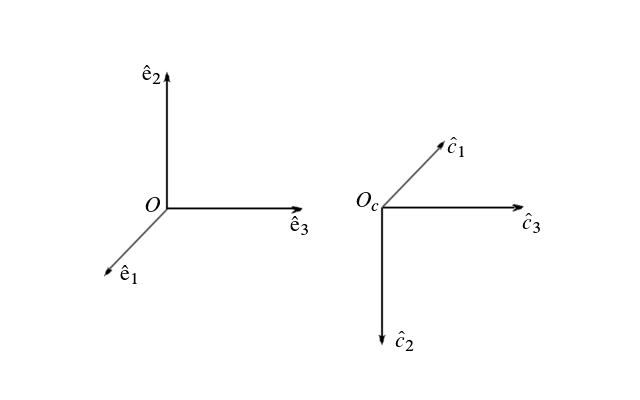
\includegraphics[width=1.\linewidth]{images/Rotation.png}
	\captionof{figure}{Weltkoordinatensystem \ensuremath{K = (O,\hat{e}_1,\hat{e}_2,\hat{e}_3)} und Kamerakoordinatensystem \ensuremath{K_c=(O_c, \hat{c}_1, \hat{c}_2, \hat{c}_3)}.}
\end{minipage}\\ \\

Zur Übersichtlichkeit wurden die Koordinatenssysteme in Abbildung 3.1 verschoben voneinander dargestellt. In Wirklichkeit sind die Ursprünge \ensuremath{O} und \ensuremath{O_c} deckungsgleich. Als nächstes werden die intrinsischen Kameraparameter festgelegt, hierbei gilt: 

\begin{gather}
\leftidx{_{K_{c}}}{\begin{bmatrix}
	\pi
	\end{bmatrix}}{_{K_{c}}} 
= 
\begin{pmatrix}
\zeta&0&0&0\\
0&\zeta&0&0\\
0&0&\zeta&0\\
0&0&1&0
\end{pmatrix}\\
\leadsto
\begin{pmatrix}
X\\Y\\Z
\end{pmatrix} = 
\leftidx{_{K_{c}}}{\begin{bmatrix}
	\pi
	\end{bmatrix}}{_{K_{c}}}
\begin{pmatrix}
X\\Y\\Z\\1
\end{pmatrix}
=
\begin{pmatrix}
\zeta X\\\zeta Y\\\zeta Z\\Z
\end{pmatrix}
=
\begin{pmatrix}
\frac{\zeta}{Z} X\\\frac{\zeta}{Z} Y\\\zeta\\1
\end{pmatrix}
\end{gather}\\

Für das Beispiel gilt zunächst die Bedingung $\zeta \neq 0$. Des Weiteren soll gelten, dass  \ensuremath{\hat{c}_3} gleich der Lotgeraden vom Sender zum Projektionszentrum entsptricht und somit folgt, dass \ensuremath{\hat{c}_1} in Sensorebene liegt und \ensuremath{\hat{c}_2 = \hat{c}_3 \times \hat{c}_1} ist. Der Quader besteht aus den Punkten $A,B,C, D$ und $E$ in homogenen Weltkoordinaten. Das Koordinatensystem von Kamera eins ist gleich dem um \ensuremath{180^\circ} gedrehte Weltkoordinatensystem. Die Punkte in Weltkoordinaten lauten wie folgt. 

\begin{gather}
(A)_K=\begin{pmatrix}
0\\0\\2\\1
\end{pmatrix}, 
(B)_K=
\begin{pmatrix}
1\\0\\2\\1
\end{pmatrix},
(C)_K=
\begin{pmatrix}
1\\1\\2\\1
\end{pmatrix},
(D)_K=
\begin{pmatrix}
0\\1\\2\\1
\end{pmatrix},
(E)_K=
\begin{pmatrix}
\frac{1}{2}\\\frac{1}{2}\\2\\1
\end{pmatrix}
\end{gather}\\

Kamera zwei wird für die Aufnahme der Szene zusätzlich noch um \ensuremath{45^\circ}zu Kamera eins eingedreht.
Für die Transformation der Weltkoordinatentupel in Kamera eins und Kamera zwei müssen also zuerst die Punkte in den jeweiligen Kamerakoordinatensystemen angegeben werden. Für die Transformation der Weltkooridinaten in die entsprechenden Kamerakoordinaten werden also zwei Matrizen \ensuremath{T_1} und \ensuremath{T_2} benötigt. \ensuremath{T_1} bewirkt die Drehung der Punkte um 180° um die \ensuremath{\hat{e}_3}-Achse. Um \ensuremath{T_2} zu erhalten wird \ensuremath{T_1} zusätzlich noch mit einer weiteren Transformationsmatrix, welche die Drehung um \ensuremath{45^\circ} beinhaltet, verrechnet. Die so erhaltenen Matrizen \ensuremath{T_1} und \ensuremath{T_2} können nun dazu verwendet werden, die Punkte Bezüglich des Weltkoordinatensystems in Punkte bezüglich der jeweiligen Kamerakoordinatensysteme zu transformieren. Im ersten Schritt erfolgt die Drehung um \ensuremath{180^\circ} um die \ensuremath{\hat{e}_3}-Achse.


\begin{gather}
	\begin{bmatrix}
		\cos(180)&-\sin(180)&0&0\\
		\sin(180)&\cos(180)&0&0\\
		0&0&1&0\\
		0&0&0&1
	\end{bmatrix}
	\begin{pmatrix}
		\hat{e}_1,\hat{e}_2,\hat{e}_3,O
	\end{pmatrix}
	=
	\begin{bmatrix}
		-1&0&0&0\\
		0&-1&0&0\\
		0&0&1&0\\
		0&0&0&1
	\end{bmatrix} 
	\begin{pmatrix}
		\hat{e}_1,\hat{e}_2,\hat{e}_3,O
	\end{pmatrix}\\
	\begin{bmatrix}
		-1&0&0&0\\
		0&-1&0&0\\
		0&0&1&0\\
		0&0&0&1
	\end{bmatrix}^T =\begin{bmatrix}
	-1&0&0&0\\
	0&-1&0&0\\
	0&0&1&0\\
	0&0&0&1
	\end{bmatrix}= T_1
\end{gather}\\

Im nächsten Schritt wird die Kamera um \ensuremath{45^\circ} zu Kamera eins eingedreht, es ergibt sich die folgende Matrix \ensuremath{T_2}:

\begin{gather}
	\cos(45)=\sin(45)=\frac{1}{\sqrt{2}} = a\\
	\begin{bmatrix}
		a&0&a&0\\
		0&1&0&0\\
		-a&0&a&0\\
		0&0&0&1
	\end{bmatrix}
	\begin{bmatrix}
		-1&0&0&0\\
		0&-1&0&0\\
		0&0&1&0\\
		0&0&0&1
	\end{bmatrix}
	=\begin{bmatrix}
		-a&0&a&0\\
		0&-1&0&0\\
		a&0&a&0\\
		0&0&0&1
	\end{bmatrix}
	\begin{pmatrix}
		\hat{e}_1,\hat{e}_2,\hat{e}_3,O
	\end{pmatrix}\\
	=\begin{bmatrix}
	-a&0&a&0\\
	0&-1&0&0\\
	a&0&a&0\\
	0&0&0&1
	\end{bmatrix}^T
	=
	\begin{bmatrix}
		-a&0&a&0\\
		0&-1&0&0\\
		a&0&a&0\\
		0&0&0&1
	\end{bmatrix}
	= T_2
\end{gather}\\


Sind die Matrizen \ensuremath{T_1} und \ensuremath{T_2} ermittelt, können nun die Weltkoordinatentupel in die Koordinatentupel von Kamera eins und Kamera zwei transformiert werden. Zunächst die transformation der Punkte in die um \ensuremath{180^\circ} gedrehte Kamera eins.

\begin{gather}
	\begin{pmatrix}
		(A)_{K_{c1}}\\1
	\end{pmatrix}
	=
	\begin{bmatrix}
		-1&0&0&0\\
		0&-1&0&0\\
		0&0&1&0\\
		0&0&0&1
	\end{bmatrix}
	\begin{pmatrix}
		0\\0\\2\\1
	\end{pmatrix}
	=
	\begin{pmatrix}
		0\\0\\2\\1
	\end{pmatrix}\\
	\begin{pmatrix}
		(B)_{K_{c1}}\\1
	\end{pmatrix}
	=
	\begin{bmatrix}
		-1&0&0&0\\
		0&-1&0&0\\
		0&0&1&0\\
		0&0&0&1
	\end{bmatrix}
	\begin{pmatrix}
		1\\0\\2\\1
	\end{pmatrix}
	=
	\begin{pmatrix}
		-1\\0\\2\\1
	\end{pmatrix}\\
	\begin{pmatrix}
		(C)_{K_{c1}}\\1
	\end{pmatrix}
	=
	\begin{bmatrix}
		-1&0&0&0\\
		0&-1&0&0\\
		0&0&1&0\\
		0&0&0&1
	\end{bmatrix}
	\begin{pmatrix}
		1\\1\\2\\1
	\end{pmatrix}
	=
	\begin{pmatrix}
		-1\\-1\\2\\1
	\end{pmatrix}\\
	\begin{pmatrix}
		(D)_{K_{c1}}\\1
	\end{pmatrix}
	=
	\begin{bmatrix}
		-1&0&0&0\\
		0&-1&0&0\\
		0&0&1&0\\
		0&0&0&1
	\end{bmatrix}
	\begin{pmatrix}
		0\\1\\2\\1
	\end{pmatrix}
	=
	\begin{pmatrix}
		0\\-1\\2\\1
	\end{pmatrix}
\end{gather}

Danach die Transformation der Weltkoordinaten in die um \ensuremath{180^\circ} um die \ensuremath{\hat{e}_3}-Achse gedrehte und zusätzlich um die \ensuremath{\hat{c}_2}-Achse um \ensuremath{45^\circ} eingedrehte Kamera zwei mit Matrix \ensuremath{T_2}.

\begin{gather}
	\begin{pmatrix}
		(A)_{K_{c2}}\\1
	\end{pmatrix}
	=
	\begin{bmatrix}
		-a&0&a&0\\
		0&-1&0&0\\
		a&0&a&0\\
		0&0&0&1
	\end{bmatrix}
	\begin{pmatrix}
		0\\0\\2\\1
	\end{pmatrix}
	=
	\begin{pmatrix}
		2a\\0\\2a\\1
	\end{pmatrix}\\
	\begin{pmatrix}
		(B)_{K_{c2}}\\1
	\end{pmatrix}
	=
	\begin{bmatrix}
		-a&0&a&0\\
		0&-1&0&0\\
		a&0&a&0\\
		0&0&0&1
	\end{bmatrix}
	\begin{pmatrix}
		1\\0\\2\\1
	\end{pmatrix}
	=
	\begin{pmatrix}
		a\\0\\3a\\1
	\end{pmatrix}\\
	\begin{pmatrix}
		(C)_{K_{c2}}\\1
	\end{pmatrix}
	=
	\begin{bmatrix}
		-a&0&a&0\\
		0&-1&0&0\\
		a&0&a&0\\
		0&0&0&1
	\end{bmatrix}
	\begin{pmatrix}
		1\\1\\2\\1
	\end{pmatrix}
	=
	\begin{pmatrix}
		a\\-1\\3a\\1
	\end{pmatrix}\\
	\begin{pmatrix}
		(D)_{K_{c2}}\\1
	\end{pmatrix}
	=
	\begin{bmatrix}
		-a&0&a&0\\
		0&-1&0&0\\
		a&0&a&0\\
		0&0&0&1
	\end{bmatrix}
	\begin{pmatrix}
		0\\1\\2\\1
	\end{pmatrix}
	=
	\begin{pmatrix}
		2a\\-1\\2a\\1
	\end{pmatrix}
\end{gather}\\

Danach müssen die entstandenen Koordinatentupel von Kamera eins und Kamera zwei noch mit ihren jeweiligen Abblildungsmatritzen verrechnet werden. $\zeta$ bekommt in diesem Beispiel den Wert -1, das bedeutet laut der Definition der Kamerakoordinatensysteme, dass der Sensor sich hinter dem Projektionszentrum befindet. Das entstehende Bild ist somit um \ensuremath{180^\circ} gespiegelt auf dem Sensor abgebildet.

\begin{gather}
	\leftidx{_{K_{c1}}}{\begin{bmatrix}
			\pi
	\end{bmatrix}}{_{K_{c1}}}
	=		\leftidx{_{K_{c2}}}{\begin{bmatrix}
			\pi
	\end{bmatrix}}{_{K_{c2}}}
	=
	\begin{pmatrix}
		\zeta&0&0&0\\
		0&\zeta&0&0\\
		0&0&\zeta&0\\
		0&0&1&0
	\end{pmatrix}=
	\begin{pmatrix}
		-1&0&0&0\\
		0&-1&0&0\\
		0&0&-1&0\\
		0&0&1&0
	\end{pmatrix}
\end{gather}

Die vier Punkte werden jeweils in einer Matrix zusammengeschrieben, so folgt für die Koordinatentupel von Kamera eins folgendes:

\begin{gather}
	\begin{pmatrix}
		-1&0&0&0\\
		0&-1&0&0\\
		0&0&-1&0\\
		0&0&1&0
	\end{pmatrix}
	\begin{pmatrix}
		0&-1&-1&0\\
		0&0&-1&-1\\
		2&2&2&2\\
		1&1&1&1
	\end{pmatrix}=
	\begin{pmatrix}
		0&1&1&0\\
		0&0&1&1\\
		-2&-2&-2&-2\\
		2&2&2&2
	\end{pmatrix}\\
	\simeq
	\begin{pmatrix}
		0&\frac{1}{2}&\frac{1}{2}&0\\
		0&0&\frac{1}{2}&\frac{1}{2}\\
		-1&-1&-1&-1\\
		1&1&1&1
	\end{pmatrix}
\end{gather}
\pagebreak

Und für die Koordinatentupel von Kamera zwei gilt:

\begin{gather}
	\begin{pmatrix}
		-1&0&0&0\\
		0&-1&0&0\\
		0&0&-1&0\\
		0&0&1&0
	\end{pmatrix}
	\begin{pmatrix}
		2a&a&a&2a\\
		0&0&-1&-1\\
		2a&3a&3a&2a\\
		1&1&1&1
	\end{pmatrix}=
	\begin{pmatrix}
		-2a&-a&-a&-2a\\
		0&0&1&1\\
		-2a&-3a&-3a&-2a\\
		2a&3a&3a&2a
	\end{pmatrix}\\
	\simeq
	\begin{pmatrix}
		-1&-\frac{1}{3}&-\frac{1}{3}&-1\\
		0&0&\frac{1}{3a}&\frac{1}{2a}\\
		-1&-1&-1&-1\\
		1&1&1&1
	\end{pmatrix}
\end{gather}\\

Die Entstandenen Punkte beider Kameras wurden in Geogebra eingegeben und das Programm liefert die folgende beide Quadrate\\

\begin{minipage}{\linewidth}
	\centering
	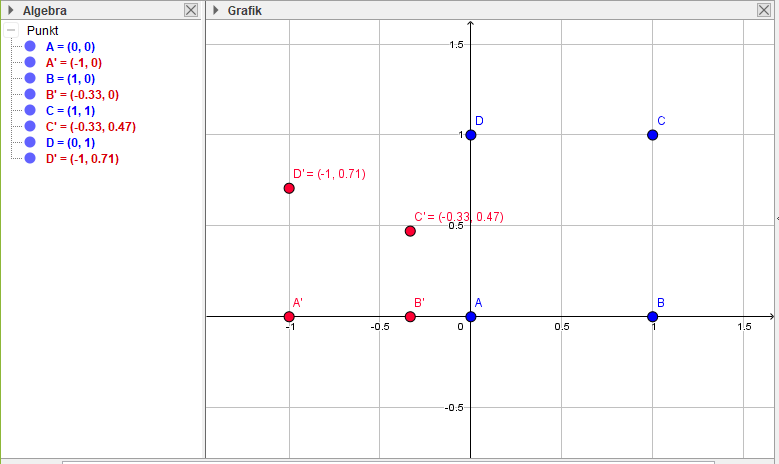
\includegraphics[width=1.\linewidth]{images/Geogebra.png}
	\captionof{figure}{in blau ist die Abblidung des Quaders von Kamera eins und in rot die Abbildung des selben Quaders in Kamera zwei (BILD NOCHMAL ÜBERARBEITEN)}
\end{minipage}\\ \\

Die nun ermittelten Punkte sollen durch eine eigens aufgestellte Homographiematrix ineinander überführt werden. Um eine Homographiematrix mit $
H=
\begin{bmatrix}
h_{11}&h_{12}&h_{13}\\
h_{21}&h_{22}&h_{23}\\
h_{31}&h_{32}&h_{33}
\end{bmatrix}
$ zu ermitteln werden die Punkte beider Kameras in eine Koeffizientenmatrix welche sich nach folgendem Schema ergibt: (Tafelaufschrieb einbauen)

\begin{gather}
\begin{bmatrix}
h_{11}&h_{12}&h_{13}\\
h_{21}&h_{22}&h_{23}\\
h_{31}&h_{32}&h_{33}
\end{bmatrix}
\cdot
\begin{bmatrix}
\\P_{K1}\\\\
\end{bmatrix}
=
\begin{bmatrix}
\\P_{K2}\\\\
\end{bmatrix}\\
\begin{bmatrix}
h_{11}&h_{12}&h_{13}\\
h_{21}&h_{22}&h_{23}\\
h_{31}&h_{32}&h_{33}
\end{bmatrix}
\cdot
\begin{bmatrix}
x\\y\\z
\end{bmatrix}
=
\begin{bmatrix}
x'\\y'\\z'
\end{bmatrix}\\
\end{gather}

Hieraus ergeben sich die folgenden drei Gleichungssysteme

\begin{gather}
h_{11}x+h_{12}y+h_{13}z= \lambda x'\\
h_{21}x+h_{22}y+h_{23}z= \lambda y'\\
h_{31}x+h_{32}y+h_{33}z= \lambda z'
\end{gather}

Da mit homogenen Koordinaten gearbeitet wird und somit $z$ und $z'$ = 1 sind, ergibt sich für die letzte Zeile $h_{31}x+h_{32}y+h_{33}z= 1$. Dieser Ausdruck kann dann in den ersten beiden Gleichungen für $\lambda$ eingesetzt werden. Es ergeben sich pro Punktepaar jeweils zwei Gleichungen. 

\begin{gather}
	h_{11}x+h_{12}y+h_{13}z= (h_{31}x+h_{32}y+h_{33}z) \cdot x'\\
		h_{21}x+h_{22}y+h_{23}z= (h_{31}x+h_{32}y+h_{33}z) \cdot y'
\end{gather}

Für den Aufbau der Koeffizientenmatrix werden beide Ausdrücke noch nach Null aufgelöst

\begin{gather}
	h_{11}x+h_{12}y+h_{13}z -(h_{31}x+h_{32}y+h_{33}z) \cdot x'= 0 \\	h_{21}x+h_{22}y+h_{23}z-(h_{31}x+h_{32}y+h_{33}z) \cdot y'=0
	\end{gather}
\begin{gather}
	\leadsto h_{11}x+h_{12}y+h_{13}z -h_{31}x\cdot x' - h_{32}y \cdot x'-h_{33}z\cdot x'= 0\\
	\leadsto h_{21}x+h_{22}y+h_{23}z-h_{31}x\cdot y -h_{32}y \cdot y -h_{33}z) \cdot y'=0
\end{gather}

Für die Koeffizientenmatrix ergibt sich dann folgendes.

\begin{gather}
	\begin{pmatrix}
	x_1&y_1&1&0&0&0&x_1 x'_1&y_1 x'_1 & 1\cdot x'_1\\
	0&0&0&x_1&y_1&1&x_1 y'_1&y_1 y'_1 & 1\cdot y'_1\\
	&&&&&.&&&\\	
	&&&&&.&&&\\	
	&&&&&.&&&\\	
	x_i&y_i&1&0&0&0&x_i x'_i&y_i x'_i & 1\cdot x'_i\\
	0&0&0&x_i&y_i&1&x_i y'_i&y_i y'_i & 1\cdot y'_i
	\end{pmatrix}
	\cdot
	\begin{pmatrix}
	h1\\h2\\.\\.\\.\\hi
	\end{pmatrix}
	=0
\end{gather}

Wenn ein Idealfall,sprich wenn der Rang der Koeffizientenmatrix genau acht beträgt, vorliegt, so kann aus der Koeffizientenmatrix einfach der Nullraum berechnet werden. Dieser Nullraum entspricht dem Kern der Koeffizientenmatrix. Das Ergebnis ist ein Spaltenvektor mit 9 Einträgen, welche in die \ensuremath{3x3}-Homographiematrix übertragen werden können. \cite{HZ}\cite{Schwarz}. Tritt nun der Fall ein, dass man ein überbestimmtes System besitzt, was auftritt wenn mehr als 9 Punktepaare durch eine Homographie ineinander überführt werden sollen, so kann nicht mehr der Nullram für die Berechnung der Homographiematrix benutzt werden. Das resultierende Ergebnis würde zwei oder mehr voneinander unabhängige Lösungen bieten, aus denen man die reale Lösung erst noch herausfinden muss. Mehr zu diesem Verfahren wird bei der Berechnung der Fundamentalmatrix nochmal genauer erläutert.\cite{HZ} Für die Lösung überbestimmter Gleichungssysteme bietet sich die Singulätwertszerlegung an\cite{HZ}\cite{Scholz}. Das bedeutet es wird nicht derjenige Vektor $x$ gesucht für den gilt $H \cdot x = 0$, sondern es wird derjenige Vektor $x$ gesucht, für den \ensuremath{\parallel H \cdot x\parallel} minimal wird.\cite{HZ}

Definition der Singulärwertszerlegung: Eine Faktorisierung einer beliebeigen Matrix \ensuremath{A \in \mathbb{R}^{mxn}} der Form \ensuremath{A = U \cdot S \cdot V^T} mit orthogonalen Matrizen \ensuremath{U \in \mathbb{R}^{m \times n}} und \ensuremath{V \in \mathbb{R}^{m \times n}} sowie mit einer Diagonalmatrix 

\begin{gather}
	S = \begin{pmatrix}
	s_1&&...&&0&0&&...&&0\\
	.&.&&&.&.&&&&.\\
	.&&.&&.&.&&&&.\\
	.&&&.&.&.&&&&.\\
	0&&...&&s_r&0&&...&&0\\	
	0&&...&&0&0&&...&&0\\
	.&&&&.&.&&&&.\\
	.&&&&.&.&&&&.\\	
	.&&&&.&.&&&&.\\	
	0&&...&&0&0&&...&&0\\	
	\end{pmatrix}
\end{gather}

heißt Singulärtwertszerlegung von $A$. Dabei gelte \ensuremath{s_1 \geq s_2 \geq ... \geq s_r \ge 0 }, und die Zahlen $s_1$ bis $s_r$ werden als Singulärwerte von $A$ bezeichnet.\cite{Scholz}.\\

(OBEN ALLES NOCH UMFORMULIEREN) \\


Entsprechend dieser Methode wird eine Singulärwertszerlegung, kurz $SVD$ der entstandenen Koeffizientenmatrix, welche gleich der Form von Matrix $A$ und im fortlaufenden auch mit $A$ bezeichnet wird, durchgeführt. Wir erhalten 3 Matrizen $U \cdot S\cdot V^T$. Durch die Zerlegung sind die diagonaleinträge von $S$ in einer absteigenden Reihenfolge sortiert. Der kleinste Sigulärwert korrespondiert auf diese Weise mit der letzten Spalte von $V$. Somit gleichen die 9 Einträge der Homographiematrix gleich der letzten Spalte von $V$. Das Ergebnis für $H$ hat dann die folgende Form

\begin{gather}
	H=
	\begin{pmatrix}
	v_{19}&v_{29}&v_{39}\\
	v_{49}&v_{59}&v_{69}\\
	v_{79}&v_{89}&v_{99}
	\end{pmatrix}
\end{gather}

Für das Minimalbeispiel mit den eigens erstellten reinen Punkten, welches in diesem Kapitel erstellt wurde, würde die Herleitung der Homographiematrix über die Ermittlung des Nullraumes der Koeffizientenmatrix genügen. Für die Matrix $H$ ergibt sich aus den Werten der im Beispiel verwendeten Punkte

\begin{gather}
	\begin{pmatrix}
	1&0&-1\\
	0&1.41421&0\\
	1&0&1
	\end{pmatrix}
\end{gather}

Nun werden die Punkte aus Kamera eins und die Punkte aus Kamera zwei jeweils mit Hilfe von $H$ ineinander überführt. Hierzu werden die Tiefenwerte $z$ der Punkte vernachlässigt. Die Punkte liegen alle auf einer Ebene, die Tiefe ist somit für die Umrechnung der Punkte nicht relevant.

\begin{gather}
		\begin{pmatrix}
	-1&-\frac{1}{3}&-\frac{1}{3}&-1\\
	0&0&\frac{1}{3a}&\frac{1}{2a}\\
	-1&-1&-1&-1\\
	1&1&1&1
	\end{pmatrix}
	=
		\begin{pmatrix}
	-1&-\frac{1}{3}&-\frac{1}{3}&-1\\
	0&0&\frac{1}{3a}&\frac{1}{2a}\\
	1&1&1&1
	\end{pmatrix}\\
		\begin{pmatrix}
	0&\frac{1}{2}&\frac{1}{2}&0\\
	0&0&\frac{1}{2}&\frac{1}{2}\\
	-1&-1&-1&-1\\
	1&1&1&1
	\end{pmatrix}
	=
		\begin{pmatrix}
	0&\frac{1}{2}&\frac{1}{2}&0\\
	0&0&\frac{1}{2}&\frac{1}{2}\\
	1&1&1&1
	\end{pmatrix}
\end{gather}

Probe:
\begin{gather}
x'=H \cdot x \leadsto 
	\begin{pmatrix}
	-1&-\frac{1}{3}&-\frac{1}{3}&-1\\
	0&0&\frac{1}{3a}&\frac{1}{2a}\\
	1&1&1&1
\end{pmatrix}= 	\begin{pmatrix}
1&0&-1\\
0&1.41421&0\\
1&0&1
\end{pmatrix}
\cdot
		\begin{pmatrix}
0&\frac{1}{2}&\frac{1}{2}&0\\
0&0&\frac{1}{2}&\frac{1}{2}\\
1&1&1&1
\end{pmatrix}
\end{gather}

und umgekehrt:

\begin{gather}
x=H^{-1} \cdot x' \leadsto 
\begin{pmatrix}
0&\frac{1}{2}&\frac{1}{2}&0\\
0&0&\frac{1}{2}&\frac{1}{2}\\
1&1&1&1
\end{pmatrix}
= 	\begin{pmatrix}
0.5&0&0.5\\
0&0.707107&0\\
0.5&0&0.5
\end{pmatrix}
\cdot
\begin{pmatrix}
-1&-\frac{1}{3}&-\frac{1}{3}&-1\\
0&0&\frac{1}{3a}&\frac{1}{2a}\\
1&1&1&1
\end{pmatrix}
\end{gather}

\section{Abbildungsunterschiede von Rotationen um ein Projektionszentrum und Rotation um einen beliebigen Drehpunkt von Punkten in der Ebene}


Im folgenden soll kurz eingeschoben werden, dass sie Abbildungen von Punkten in einer Ebene unterscheiden, sobald sich ihr Drehpunkt ändert. Zu diesem Zweck wurde eine kleine Simulation geschrieben, welche die Abbildung eines Objekts zeigt, wenn sich die Kamera um ihr Kamerazentrum dreht und im Vergleich hierzu wenn sie sich um einen definierten Drehpunkt dreht. In diesem Beispiel ist der rote Punkte der Drehpunkt. Die Frage die sich hinter dieser Simulation befand war, ob es bei beiden Drehungen zum selben oder unterschiedlichen Bildern kommt. Des Weiteren sollte geklärt werden, ob Punkte die bei der Drehung um das Projektionszentrum verdeckt bleiben auch bei einer Drehung um einen außerhalb der Kamera platzierten Drehpunkt ebenfalls verdeckt bleiben und ob eine gültige Homographiematrix errechnet werden kann. Abbildung 3.3 zeigt ein Quadrat mit vier Eckpunkten und seinem Mittelpunkt in rot.

\begin{minipage}{\linewidth}
	\centering
	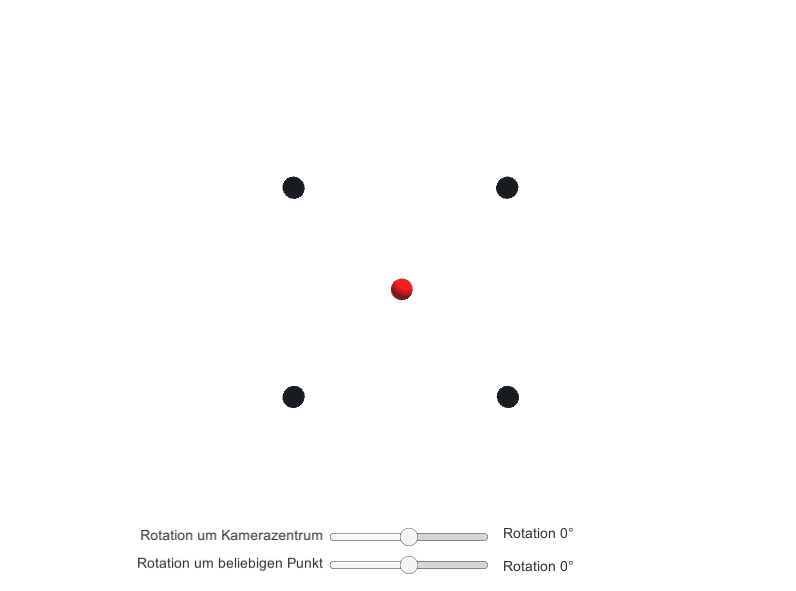
\includegraphics[width=.8\linewidth]{images/Ausgangslage.png}
	\captionof{figure}{Objekt im Raum}
\end{minipage}\\


Für die Simulation der Drehung wurden zwei Schieberegler implementiert mit dem sich die Kamera einmal um ihre eigene y-Achse in diesem Fall das Projektionszentrum dreht und einmal um den Drehpunkt, welche wie bereits gesagt der rote Mittelpunkt ist.


\begin{minipage}{\linewidth}
	\centering
	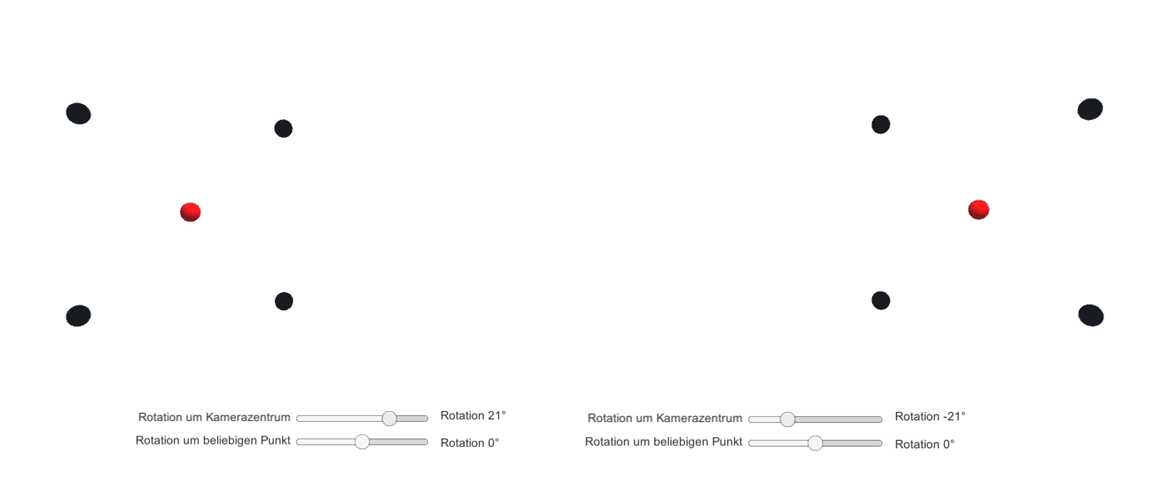
\includegraphics[width=1.\linewidth]{images/DrehungPZ.png}
	\captionof{figure}{Drehung um das Projektionszentrum}
\end{minipage}\\ \\

Abblidung 4.3 zeigt jeweils die entstehende Abbildung wenn die Kamera um \ensuremath{20^\circ} beziehungsweise \ensuremath{-20^\circ} um das Projektionszentrum gedreht wurde.

\begin{minipage}{\linewidth}
	\centering
	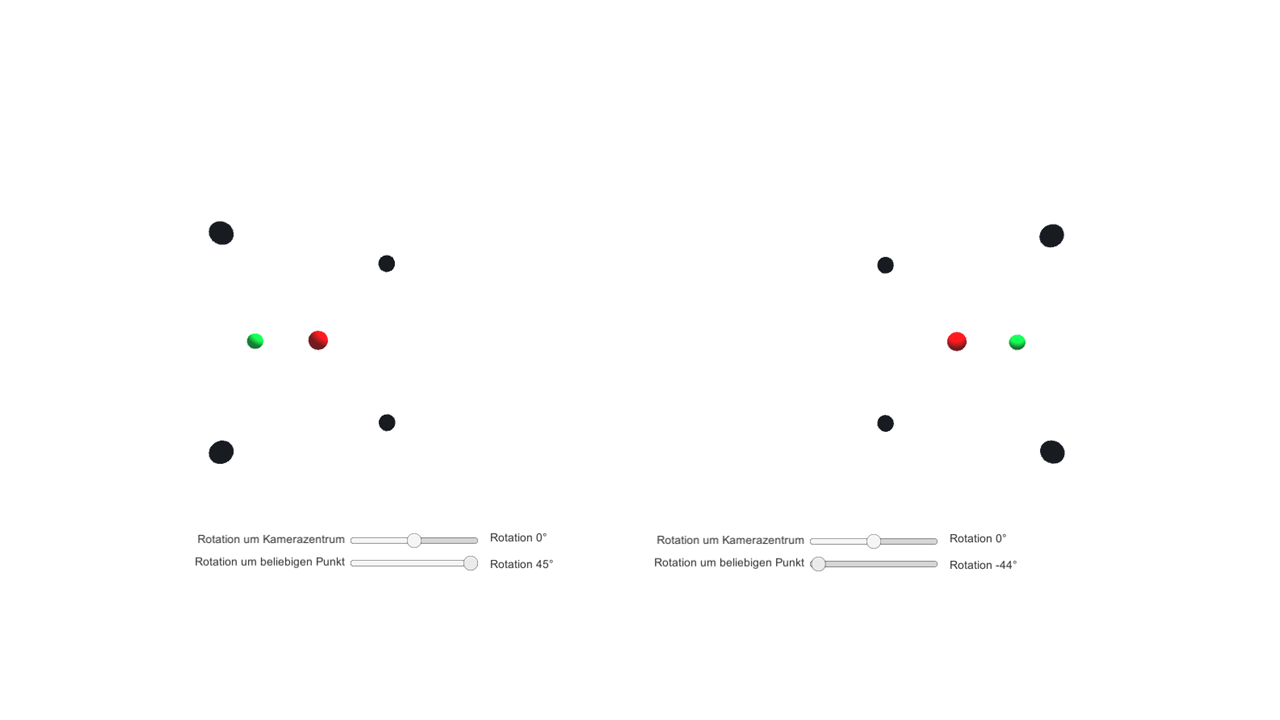
\includegraphics[width=1.\linewidth]{images/DrehungDZ.png}
	\captionof{figure}{Drehung um einen Drehpunkt. In diesem Beispiel wurde der rote Punkt als Drehpunkt verwendet}
\end{minipage}\\ \\

Abbildung 3.4 zeigt die entstehenden Bilder, wenn die Kamera um \ensuremath{45^\circ} beziehungsweise \ensuremath{-45^\circ} um den Drehpunkt gedreht wurde. Wie sich zeigt ist hier der Punkt welcher hinter dem roten Punkt platziert wurde sichtbar. Die Behauptung die nun noch zu beweisen gilt ist, dass die jeweilingen Abblidungen beide Drehungen durch jeweils eine Homographiematrix $H$ dargestellt werden können, sofern sich die Punkte auf einer Ebene befinden. Ausgegangen wird immer vom Ursprungsbild in Abblidung 3.3. Das die Drehung um das Projektionszentrum eine gültige Homographiematrix hervorbringt wurde im vorherigen Unterkapitel (Link Kapitel 3.1) bereits gezeigt. Die Herangehensweise für das Beispiel um einen Drehpunkt ist die größtenteils die selbe. Das einzige was sich unterscheidet ist die Transformation der Punkte in as Koordinatensystem von Kamera zwei. Diese besteht hier nicht nur aus einer Rotation, sondern zu allererst wird die Kamera zwei zum Drehpunkt verschoben, dann gedreht und zum Schluss wieder um den selben Translatationvektor zurückverschoben. Die Transformationsmatrix $M$ hat besteht dann aus drei Transformationsmatrizen \ensuremath{M = V_1 \cdot R \cdot V_2}. \\


Beispiel aufzeigen (Code)\\

Beweis Homographie (beinhaltet sowohl Translation als auch Rotation)--> Drehung um ein Drehpunkt ist nichts weiter als eine Translation + Rotation und Rücktranslation. --> Punkte bleiben auf einer Ebene--> alle Vorraussetzungen für Homographien sind erfüllt\\



 Sollte wie im zweiten Beispiel der grüne Punkte mit durch eine Homographie übermittelt werden, so ist die entstehende Homographie ungültig. Kamera zwei ist in diesem Beispiel um ihr Projektionszentrum gedreht.\\



--> erklären warum homographien nur in der Ebene funktionieren


\section{Punkte in unterschiedlichen Ebenen}

Überleitung zur Epipolargeometry.\\
Warum kann hier keine Homographie benötigt werden\\
was muss hier genutzt werden?

\section{Epipolargeometrie als Grundlage der Stereokalibrierung und Szenenrekonstrunktion}


(MEHR LITERATUR FINDEN ZUM VERGLEICHEN)

\section{Geometrische Erläuterung der Fundamentalmatrix und der Essentiellen Matrix }







